\documentclass{article}
\usepackage[spanish, es-tabla]{babel}
\usepackage[utf8]{inputenc}
\setlength\parindent{0pt}
\usepackage{booktabs}     % tablas 
\usepackage{multirow}
\usepackage{tabulary}     % tablas
\usepackage{float}         % para fijar las imagenes con h y H
\usepackage{graphicx}      % poner imagenes 
\usepackage{makeidx}         % allows index generation
\usepackage{multicol}        % used for the two-column index
\usepackage[bottom]{footmisc}% places footnotes at page bottom



\usepackage{Sweave}
\begin{document}
\Sconcordance{concordance:informe_digitos.tex:informe_digitos.Rnw:%
1 15 1 1 0 76 1 1 3 2 0 1 5 4 0 1 2 5 0 1 3 31 1 1 2 1 0 1 2 1 0 1 3 2 %
0 1 3 5 0 1 2 72 1 1 2 1 0 1 2 4 0 1 2 48 1 1 3 2 0 1 2 1 0 2 1 3 0 1 2 %
97 1 1 3 2 0 1 3 2 0 1 4 5 0 1 2 80 1 1 2 1 0 1 7 6 0 1 8 10 0 1 3 38 1 %
1 14 13 0 1 8 10 0 1 3 108 1}


\author{Heber Esteban Bermúudez \\
John Bryan Yepez \\
Simon Zapata}
\title{MODELOS ESTADÍSTICOS PARA LA CLASIFICACIÓN DE DÍGITOS \\
{\small Universidad Nacional de Colombia - Sede Medellín}}
\maketitle

\begin{abstract}
\noindent
En este trabajo se aborda la construcción de modelos de clasificación multiclase para predecir la clasificación de dígitos, esto se hizo usando el conjunto de datos MNIST que es una gran base de datos de dígitos escritos a mano.\\
Las metodologías que se abordaron para construir los modelos son las siguientes. \\
1. Regresión logística multinomial\\
2. Árboles de clasificación\\
3. Bosques aleatorios\\
4. Máquinas de soporte vectorial\\
5. Redes neuronales\\
El objetivo es validar y comparar los cinco métodos de clasificación mencionados bajo distintas configuraciones de sus parámetros o métodos para luego elegir el modelo de mejor rendimiento usando como críterio la tasa de clasificación correcta de dígitos sobre datos de prueba.
\end{abstract}


\section{Definiciones}

\textbf{MNIST}\\
La base de datos MNIST (base de datos modificada del Instituto Nacional de Estándares y Tecnología) es una gran base de datos de dígitos escritos a mano que se usa comúnmente para capacitar a varios sistemas de procesamiento de imágenes. La base de datos también se usa ampliamente para capacitación y pruebas en el campo del aprendizaje automático.\\

\textbf{Modelo Estadístico}\\
El modelado estadístico es una forma simplificada, matemáticamente formalizada para aproximarse a la realidad que genera los datos) y, opcionalmente, hacer predicciones a partir de dicha aproximación.


\section{Metodología}
En el presente trabajo se bordan las metodologías estadísticas más ampliamente usadas en el campo del aprendizaje automático supervisado, para entrenar distintos modelos de clasificación, con distintos métodos o configuraciones con el objetivo de clasificar dígitos del conjunto de datos MNIST. Por cada modelo mostrado y sus distintas configuraciones, se muestra el rendimiento de este haciendo uso de la tasa de clasificación correcta sobre el conjunto de datos de prueba (test) que es un subconjunto de la base original MNIST. se usó el lenguaje estadístico R para hacer estos análisis.  

\subsection{Análisis descriptivo}

Antes de iniciar mostramos un breve análisis estadístico de las bases de datos a usar en el desarrollo del trabajo.\\

Dimensión de la base de datos de entrenamiento (trainingData)

\begin{table}[ht]
	\caption{\small{Dimensión de la base de datos trainingData.}}
	\label{tabla1}
	\centering {\small
	\begin{tabular}{@{}cc@{}}
		\toprule
		Número de Filas & Número de Columnas \\ \midrule
		 60000            & 785                 \\ \bottomrule
	\end{tabular}}
\end{table}

Dimensión de la base de datos de prueba (testingData)

\begin{table}[ht]
	\caption{\small{Dimensión de la base de datos testingData.}}
	\label{tabla1}
	\centering {\small
	\begin{tabular}{@{}cc@{}}
		\toprule
		Número de Filas & Número de Columnas \\ \midrule
		 10000            & 785                 \\ \bottomrule
	\end{tabular}}
\end{table}

Cada fila representa un dígito con la primera columna como la etiqueta de ese digito y las columnas restantes los pixeles de este y cada observación de las variables con el valor del pixel.\\

A continuación en la Figura 1 se muestra la imagen de uno de los dígitos.

\begin{figure}[H]
    \centering
	
\includegraphics{figure/digito.png}
	\caption{Observación 10 de la base de datos trainingData}
\end{figure}

Se uso el siguiente código para graficar la observación.

\begin{Schunk}
\begin{Sinput}
> #Ver uno de los digitos como imagen
> library(magick)
> im <- function(x,m){ #Funcion para ver el digito
+   plot(image_read(aperm(array(as.numeric(m[x,2:785]),c(28,28,1)),
+                         c(2,1,3)))) #Muestra la imagen en el viewer
+   return(m[x,1]) #Muestra el numero respectivo en consola
+ }
> #Imagen 1 de trainingData
> im(10,trainingData)
> 
\end{Sinput}
\end{Schunk}


En la Figura 2 se muestra la distribución de los dígitos en la base de datos de entrenamiento (trainingData).

\begin{figure}[H]
    \centering
	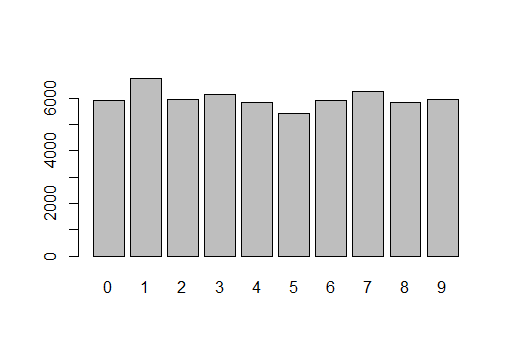
\includegraphics{figure/entrena.png}
	\caption{Distribución de los dígitos en la base de datos de entrenamiento (trainingData)}
\end{figure}



En la Figura 3 se muestra la distribución de los dígitos en la base de datos de prueba (testingData).

\begin{figure}[H]
    \centering
	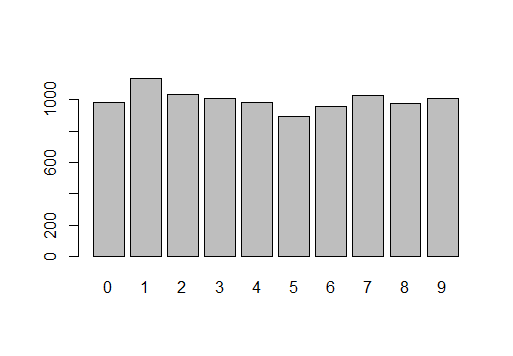
\includegraphics{figure/test.png}
	\caption{Distribución de los dígitos en la base de datos de prueba (testingData)}
\end{figure}

Se ve que la cantidad de dígitos por cada nivel tiene distribución uniforme en cada base de datos.



\subsection{Regresión logística multinomial}

La regresión logística multinomial generaliza el método de regresión logística para problemas multiclase, es decir, se trata de un modelo que se utiliza para predecir las probabilidades de los diferentes resultados posibles de una distribución categórica como variable dependiente, en nuestro caso tenemos 10 categorías correspondientes a los dígitos del 0 al 9.

Para este modelo se hizo uso de la libreria nnet() de R, y se probaron 3 modelos con distintos número de iteraciones y criterio de ajuste o tolerancia 'abstol'.

A continuación se muestra el código R con el que se construyeron los modelos. 

\begin{Schunk}
\begin{Sinput}
> library(nnet)
> # máximo número de iteraciones igual a 100 (por defecto)
> lm_1 <- multinom(V1 ~ .,data = trainingData, MaxNWts = 7860)
> # máximo número de iteraciones igual a 200 (maxit=200)
> lm_2 <- multinom(V1 ~ .,data = trainingData, MaxNWts = 7860, 
+                 maxit = 200)
> # máximo número de iteraciones igual a 200 (maxit=200) y tolerancia de 1.e-8
> lm_3 <- multinom(V1 ~ .,data = trainingData, MaxNWts = 7860,
+                 maxit = 200, abstol = 1.e-8)
\end{Sinput}
\end{Schunk}

Los resultados de la regresión logística multinomial con número máximo de iteración igual a 100 se muestra en la Tabla 3, donde presenta un rendimiento en cuanto a tasa de clasificación correcta de dígitos del 89.76\% para la base de prueba testingData

\begin{table}[H]
\caption{\small{Matriz de confusión Modelo 1 - logístico multinomial}}
\centering
\begin{tabular}{r|rrrrrrrrrr}
  \hline
 & 0 & 1 & 2 & 3 & 4 & 5 & 6 & 7 & 8 & 9 \\ 
  \hline
0 & 920 &   0 &   1 &   1 &   3 &  30 &  16 &   2 &   6 &   1 \\ 
  1 &   0 & 1118 &   3 &   3 &   1 &   1 &   4 &   1 &   4 &   0 \\ 
  2 &   7 &  15 & 915 &  10 &  10 &   6 &  17 &   8 &  39 &   5 \\ 
  3 &   9 &   3 &  26 & 888 &   5 &  19 &   7 &  10 &  35 &   8 \\ 
  4 &   0 &   9 &   2 &   2 & 917 &   1 &  11 &   3 &   4 &  33 \\ 
  5 &  11 &  10 &   2 &  34 &  12 & 668 &  35 &  10 & 102 &   8 \\ 
  6 &   5 &   7 &   6 &   0 &   8 &  12 & 919 &   1 &   0 &   0 \\ 
  7 &   4 &  26 &  23 &   2 &  11 &   1 &   2 & 916 &   5 &  38 \\ 
  8 &   5 &  33 &   9 &  13 &  11 &  21 &  14 &  10 & 847 &  11 \\ 
  9 &   3 &   9 &   0 &  10 &  70 &   6 &   6 &  22 &  15 & 868 \\ 
   \hline
\end{tabular}
\end{table}



Los resultados de la regresión logística multinomial con número máximo de iteración igual a 200 se muestra en la Tabla 4, donde presenta un rendimiento en cuanto a tasa de clasificación correcta de dígitos del 78.63\% para la base de prueba testingData


\begin{table}[H]
\caption{\small{Matriz de confusión Modelo 2 - logístico multinomial}}
\centering
\begin{tabular}{r|rrrrrrrrrr}
  \hline
 & 0 & 1 & 2 & 3 & 4 & 5 & 6 & 7 & 8 & 9 \\ 
  \hline
0 & 745 &   9 &  47 &   6 &   5 &  89 &  16 &  33 &  14 &  16 \\ 
  1 &   2 & 1091 &   7 &   9 &   5 &   2 &   7 &   1 &  10 &   1 \\ 
  2 &   7 &  36 & 770 &  52 &  16 &  14 &  26 &  41 &  55 &  15 \\ 
  3 &   6 &   8 &  30 & 773 &  10 &  78 &   6 &  45 &  27 &  27 \\ 
  4 &   4 &  16 &   8 &   8 & 818 &   7 &  18 &  27 &  26 &  50 \\ 
  5 &  14 &  17 &  16 &  36 &  23 & 648 &  28 &  21 &  55 &  34 \\ 
  6 &  17 &  17 &  45 &   2 &  63 &  27 & 737 &  14 &  18 &  18 \\ 
  7 &   3 &  26 &  31 &  16 &  17 &  10 &   6 & 861 &   7 &  51 \\ 
  8 &   8 &  45 &  50 &  34 &  26 &  71 &  17 &  31 & 649 &  43 \\ 
  9 &   3 &  15 &  12 &   9 &  80 &  20 &   7 &  78 &  14 & 771 \\ 
   \hline
\end{tabular}
\end{table}


%------------------------------------------------------------------

\subsection{Arboles de clasificación}

Los Árboles de clasificación son modelos de predicción que pueden usarse tanto para clasificación como para regresión, y cuyo funcionamiento se basa en la construcción de reglas lógicas para dividir los datos entre rangos mediante condiciones.\\
Un ejemplo práctico es como se muestra a continuación en la Figura 4 donde se realiza un árbol de clasificación para decidir si jugar o no jugar golf con  P=jugar y N= no jugar.



\begin{figure}[H]
    \centering
	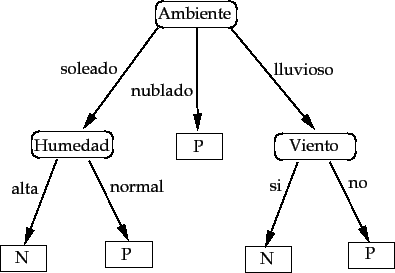
\includegraphics[scale=0.5]{figure/arboles1.png}
	\caption{Ejemplo de árbol de clasificación}
\end{figure}




Para este modelo se hizo uso de la librería rpart() de R, que permite elegir entre los método “class” para clasificación, método "$\exp$" si la variable respuesta en un objeto de supervivencia, método  "poisson"  si la variable respuesta tiene dos columnas.\\
\\
Para este conjunto de datos en particular se hizo uso método “class”, con vector de costos constante para cada variable, a continuación se muestra el código R para el modelo.  
\\
\begin{Schunk}
\begin{Sinput}
> library(rpart)
> # Arboles de clasifiación con los metodos class
> modelo1_rpart <- rpart(V1 ~ ., data = trainingData, method = "class")
\end{Sinput}
\end{Schunk}

En Tabla 5 se muestra la matriz de confusión obtenida con el modelo de árboles de regresión y método class sobre el conjunto de datos de prueba testingData, en la diagonal principal de la matriz se observan las clasificaciones correctas por cada digito, donde se puede concluir que el rendimiento de este modelo en cuanto a tasa de clasificación de observaciones correctas es de  aproximadamente 61\%

\begin{table}[H]
\caption{\small{Matriz de confusión Arboles de clasificación método class}}
\centering
\begin{tabular}{r|rrrrrrrrrr}
  \hline
 & 0 & 1 & 2 & 3 & 4 & 5 & 6 & 7 & 8 & 9 \\ 
  \hline
0 & 793 &   4 &   1 &   9 &   6 &  35 &  52 &  55 &  10 &  15 \\ 
  1 &   2 & 964 &  35 &  56 &   0 &   0 &   0 &  10 &  67 &   1 \\ 
  2 &  72 &  83 & 511 &  61 &  19 &   1 &  54 &  82 & 134 &  15 \\ 
  3 &  23 &  20 &  35 & 651 &   7 & 101 &  23 &  20 & 110 &  20 \\ 
  4 &   5 &  32 &   6 &  13 & 608 &  30 & 103 &  61 &  59 &  65 \\ 
  5 &  70 &  30 &   8 & 100 &  53 & 221 & 125 &  21 & 191 &  73 \\ 
  6 &  33 &  39 &  50 &  35 &  69 &  36 & 570 &  38 &  84 &   4 \\ 
  7 &   2 &  14 &  36 &   6 &  31 &  24 &   5 & 793 &  61 &  56 \\ 
  8 &  12 &  76 &  38 &  75 &  21 & 131 &  64 &   6 & 519 &  32 \\ 
  9 &   6 &  17 &   2 &  17 &  39 & 125 &  44 &  86 & 107 & 566 \\ 
   \hline
\end{tabular}
\end{table}


% hay que hacer otro modelito con rpart usando otra configuración




% ******************************************************************

\subsection{Bosques aleatorios}

La clasificación con Bosques Aleatorios implica la construcción de una gran cantidad de árboles de clasificación sobre un el conjunto de datos y por tanto incurre en un gran gasto computacionalmente.\\

En la Figura 5 se muestra que un Bosque aleatorio es una construcción de varios árboles de clasificación como se mostró en el ejemplo anterior.

\begin{figure}[H]
    \centering
	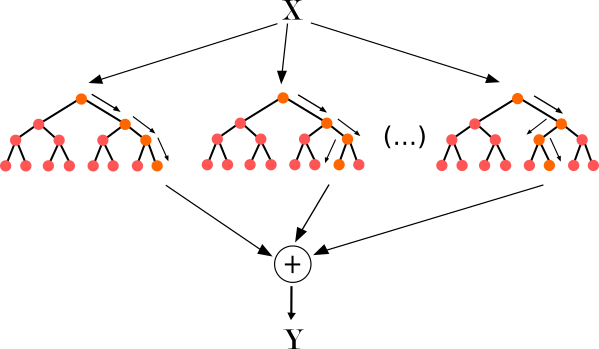
\includegraphics[scale=0.5]{figure/bosques1.png}
	\caption{Ejemplo de Bosque aleatorio.}
\end{figure}

Donde $X$ representan las variables regresaras o datos de entrada y $Y$ los datos de salida o respuesta del modelo.

Para implementar el Random Forest sobre nuestros datos MNIST se empleo la función randomForest del paquete randomForest con 10, 100 y 200 árboles, los resultados se muestran a continuación.\\

El código empleado para la construcción de los modelos es como sigue. 
\begin{Schunk}
\begin{Sinput}
> # cargando libreria al ambiente de trabajo
> library(randomForest)
> # construccion con 10 árboles
> clasificadorRF1 <- randomForest(V1 ~ ., data = trainingData, ntree = 10)
> clasificadorRF2 <- randomForest(V1 ~ ., data = trainingData, ntree = 100)
> clasificadorRF3 <- randomForest(V1 ~ ., data = trainingData, ntree = 200)
\end{Sinput}
\end{Schunk}


Con 10 árboles se obtiene una tasa de clasificación correcta de dígitos de aproximadamente el 94.91 \% para los datos de prueba testingData como se  muestra en la Tabla 6.

\begin{table}[H]
\caption{\small{Matriz de confusión Bosques aleatorios con 10 árboles}}
\centering
\begin{tabular}{r|rrrrrrrrrr}
  \hline
 & 0 & 1 & 2 & 3 & 4 & 5 & 6 & 7 & 8 & 9 \\ 
  \hline
0 & 967 &   1 &   1 &   1 &   0 &   2 &   5 &   1 &   2 &   0 \\ 
  1 &   0 & 1117 &   4 &   2 &   0 &   2 &   4 &   1 &   4 &   1 \\ 
  2 &   6 &   2 & 976 &   7 &   5 &   3 &   8 &  13 &   9 &   3 \\ 
  3 &   2 &   1 &  12 & 949 &   0 &  20 &   3 &  11 &  11 &   1 \\ 
  4 &   1 &   1 &   4 &   0 & 930 &   1 &   8 &   1 &  10 &  26 \\ 
  5 &   6 &   1 &   4 &  28 &   6 & 826 &   8 &   1 &   7 &   5 \\ 
  6 &  10 &   3 &   5 &   0 &   6 &  12 & 918 &   0 &   4 &   0 \\ 
  7 &   3 &   7 &  21 &   5 &   4 &   1 &   0 & 961 &   5 &  21 \\ 
  8 &   5 &   1 &   6 &  14 &   9 &  15 &   8 &   2 & 903 &  11 \\ 
  9 &   3 &   5 &   3 &  11 &  19 &   5 &   2 &   4 &  13 & 944 \\ 
   \hline
\end{tabular}
\end{table}


Los resultados obtenidos usando 100 árboles nos muestra que para el conjunto de validación se obtiene una tasa de clasificación de observaciones correctas del 96,92\% para los datos de prueba testingData como se muestra en la siguiente matriz de confusión ver Tabla 7.

\begin{table}[H]
\caption{\small{Matriz de confusión Bosques aleatorios con 100 árboles}}
\centering
\begin{tabular}{r|rrrrrrrrrr}
  \hline
 & 0 & 1 & 2 & 3 & 4 & 5 & 6 & 7 & 8 & 9 \\ 
  \hline
0 & 972 &   1 &   1 &   0 &   0 &   2 &   2 &   1 &   1 &   0 \\ 
  1 &   0 & 1124 &   2 &   3 &   0 &   2 &   2 &   0 &   1 &   1 \\ 
  2 &   6 &   0 & 999 &   6 &   2 &   1 &   2 &  10 &   6 &   0 \\ 
  3 &   1 &   0 &  11 & 967 &   0 &  10 &   0 &  10 &  10 &   1 \\ 
  4 &   2 &   0 &   0 &   0 & 957 &   0 &   5 &   0 &   2 &  16 \\ 
  5 &   2 &   0 &   1 &   9 &   2 & 865 &   4 &   1 &   6 &   2 \\ 
  6 &   9 &   3 &   0 &   0 &   4 &   5 & 932 &   0 &   5 &   0 \\ 
  7 &   1 &   3 &  21 &   0 &   0 &   0 &   0 & 991 &   3 &   9 \\ 
  8 &   4 &   0 &   6 &  11 &   6 &   4 &   4 &   3 & 925 &  11 \\ 
  9 &   5 &   6 &   1 &  10 &  13 &   2 &   1 &   5 &   6 & 960 \\ 
   \hline
\end{tabular}
\end{table}


Los resultados obtenidos para un conjunto de 200 árboles se muestra a continuación (ver Tabla 8). 
y presenta 97.1 \% de  tasa de clasificación correcta de dígitos sobre la base de datos de prueba testingData. 

\begin{table}[H]
\caption{\small{Matriz de confusión Bosques aleatorios con 200 árboles}}
\centering
\begin{tabular}{r|rrrrrrrrrr}
  \hline
 & 0 & 1 & 2 & 3 & 4 & 5 & 6 & 7 & 8 & 9 \\ 
  \hline
0 & 968 &   0 &   0 &   0 &   0 &   2 &   4 &   1 &   4 &   1 \\ 
  1 &   0 & 1123 &   3 &   3 &   0 &   2 &   2 &   0 &   1 &   1 \\ 
  2 &   6 &   0 & 998 &   6 &   3 &   0 &   4 &   9 &   6 &   0 \\ 
  3 &   0 &   0 &   7 & 977 &   0 &   7 &   0 &   9 &   8 &   2 \\ 
  4 &   1 &   0 &   0 &   0 & 956 &   0 &   5 &   0 &   3 &  17 \\ 
  5 &   2 &   0 &   1 &  13 &   3 & 860 &   4 &   2 &   5 &   2 \\ 
  6 &   7 &   3 &   0 &   0 &   3 &   4 & 936 &   0 &   5 &   0 \\ 
  7 &   1 &   3 &  18 &   2 &   0 &   0 &   0 & 990 &   2 &  12 \\ 
  8 &   3 &   0 &   5 &   7 &   4 &   6 &   3 &   4 & 935 &   7 \\ 
  9 &   5 &   5 &   2 &   8 &   9 &   1 &   1 &   4 &   7 & 967 \\ 
   \hline
\end{tabular}
\end{table}

Se observa que a medida que aumentamos el número de árboles aumenta la precisión del modelo en cuanto a tasa de clasificación correcta para los datos de prueba testingData. 



%***************************************************

\subsection{Máquinas de soporte vectorial}

Las Máquinas de soporte vectorial son modelos capaces de generar clasificaciones de datos no lineales a partir de la transformación de los datos de entrada a otros espacios de mayores dimensiones, con fin de encontrar una dimensión donde las observación serán separables de la mejor manera, Las SVM busca encontrar aquella curva que sea capaz de separar y clasificar los datos de entrenamiento garantizando que la separación entre ésta y ciertas observaciones del conjunto de entrenamiento (los vectores de soporte) sea la mayor posible, aunque esta metodología es más recomendada para clasificación binaria, en este ejemplo de la clasificación de dígitos la usaremos esta metodología como un modelo multiclase.\\

En la Figura 6 se muestra la ilustración del objetivo de las máquinas de soporte vectorial el cual es encontrar la una recta en el caso de 2 dimensiones donde las observaciones divididas en 2 clase sean separables de la mejor manera posible.

\begin{figure}[H]
    \centering
	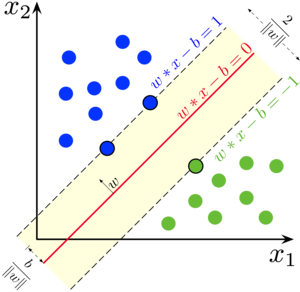
\includegraphics[scale=2.9]{figure/svm.png}
	\caption{Ejemplo de maquina de soporte vectorial.}
\end{figure}

La clase 1 es representada con el color azul y la clase 2 con el color verde en función de dos variables regresoras $x1$ y $x2$. \\

Los métodos usados en las SVM son el kernel 'linear', 'polynomial', 'sigmoid' y 'radial basis' se comprarán los primeros 2 métodos con costo de violación de las restricciones constantes en 1 y con criterio de tolerancia de terminación (por defecto: 0.001). \\

El código empleado para la creación de los modelos se muestra a continuación.

\begin{Schunk}
\begin{Sinput}
> # cargando la librería al ambiente de trabajo
> library(e1071)
> # hacemos uso de la función svm con kernel lineal y tipo clasificación
> clasificadorSVM_lineal <- svm(V1 ~ ., data = trainingData, 
+                        type = 'C-classification', kernel = 'linear')
> # hacemos uso de la función svm con kernel polynomial y tipo clasificación
> clasificadorSVM_polynomial <- svm(V1 ~ ., data = trainingData, 
+                               type = 'C-classification', kernel = 'polynomial')
\end{Sinput}
\end{Schunk}




Para el método 'linear' se obtuvo una tasa de clasificación correcta del 90.86\% la matriz de confusión se muestra a continuación (ver Tabla 9).

\begin{table}[H]
\caption{\small{Matriz de confusión Máquinas de soporte vectorial método 'linear'}}
\centering
\begin{tabular}{r|rrrrrrrrrr}
  \hline
 & 0 & 1 & 2 & 3 & 4 & 5 & 6 & 7 & 8 & 9 \\ 
  \hline
0 & 940 &   0 &   4 &   3 &   2 &  11 &  10 &   3 &   2 &   5 \\ 
  1 &   0 & 1109 &   1 &   2 &   0 &   1 &   5 &   0 &  17 &   0 \\ 
  2 &   7 &   7 & 905 &  29 &  12 &   4 &  17 &  12 &  35 &   4 \\ 
  3 &   2 &   2 &  19 & 901 &   1 &  27 &   3 &  14 &  25 &  16 \\ 
  4 &   1 &   0 &   4 &   0 & 914 &   0 &  13 &   7 &   2 &  41 \\ 
  5 &   7 &   7 &   6 &  42 &   5 & 747 &  18 &   3 &  43 &  14 \\ 
  6 &   7 &   2 &   9 &   1 &   6 &   9 & 918 &   0 &   6 &   0 \\ 
  7 &   0 &   8 &  21 &   7 &   7 &   0 &   0 & 910 &  11 &  64 \\ 
  8 &  10 &   5 &  10 &  27 &   9 &  27 &   8 &   5 & 855 &  18 \\ 
  9 &   3 &   6 &   1 &   6 &  46 &   9 &   0 &  39 &  12 & 887 \\ 
   \hline
\end{tabular}
\end{table}




Para el método 'polynomial' se obtuvo una tasa de clasificación correcta del 97.91\% la matriz de confusión se muestra a continuación (ver Tabla 10)

\begin{table}[H]
\caption{\small{Matriz de confusión Máquinas de soporte vectorial método 'polynomial'}}
\centering
\begin{tabular}{r|rrrrrrrrrr}
  \hline
 & 0 & 1 & 2 & 3 & 4 & 5 & 6 & 7 & 8 & 9 \\ 
  \hline
0 & 972 &   0 &   1 &   0 &   0 &   3 &   1 &   0 &   2 &   1 \\ 
  1 &   0 & 1124 &   2 &   1 &   1 &   2 &   3 &   0 &   2 &   0 \\ 
  2 &   7 &   0 & 1006 &   0 &   2 &   1 &   5 &   7 &   3 &   1 \\ 
  3 &   0 &   2 &   1 & 987 &   0 &   6 &   0 &   5 &   6 &   3 \\ 
  4 &   2 &   0 &   2 &   0 & 965 &   0 &   3 &   1 &   0 &   9 \\ 
  5 &   2 &   0 &   0 &   7 &   1 & 870 &   3 &   0 &   4 &   5 \\ 
  6 &   4 &   5 &   1 &   0 &   3 &   6 & 937 &   0 &   2 &   0 \\ 
  7 &   0 &   9 &   9 &   2 &   2 &   0 &   0 & 1000 &   0 &   6 \\ 
  8 &   5 &   0 &   1 &   2 &   4 &   4 &   1 &   4 & 950 &   3 \\ 
  9 &   3 &   5 &   0 &   3 &   9 &   4 &   1 &   1 &   3 & 980 \\ 
   \hline
\end{tabular}
\end{table}

Se puede observar que el modelo con kernel 'polynomial' presenta mayor rendimiento que el modelo con kernel 'linear' en cuanto a tasa de clasificación correcta para el conjunto de datos de prueba.




%------------------------------------------------------------------------------------------

\subsection{Redes neuronales}

Una red neuronal convolucional es un tipo de red neuronal artificial donde las neuronas corresponden a campos receptivos de una manera muy similar a las neuronas en la corteza visual primaria de un cerebro biológico, estas son muy efectivas para tareas de visión artificial, como en la clasificación y segmentación de imágenes, entre otras aplicaciones, en este desarrollo probaremos dos diferentes configuraciones de redes neuronales convulucionales.

En la Figura 7 se muestra una estructura de una red neuronal con 2 capas ocultas nodos de color verde y cuatro variables de entrada nodos de color rojo y tres variables respuesta color morado.  

\begin{figure}[H]
    \centering
	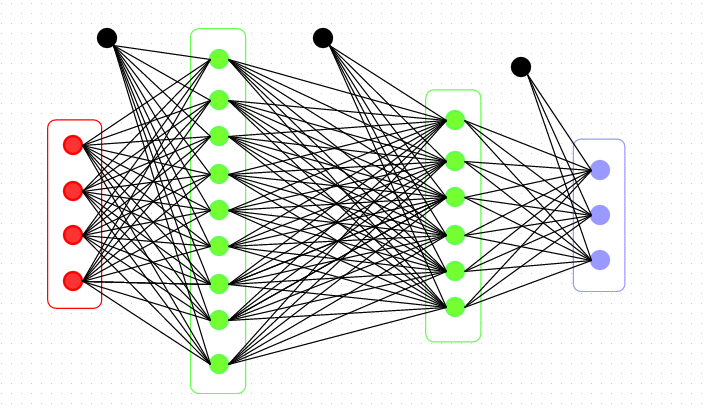
\includegraphics[scale=0.5]{figure/redes.png}
	\caption{Estructura de una Red neuronal Artificial}
\end{figure}

Para el desarrollo de este trabajo se hizo uso de la librearía keras de R para el manejo de redes neuronales artificiales.\\

Para la primera configuración de la red se tomó para la capa de entrada 10 nodos uno por cada digito o clase y se usaron dos capas ocultas una con 512 nodos y la otra con 128 nodos agregando como funcion de activación 'relu' para cada capa oculta, para esta arquitectura se usó el modelo secuencial del keras. 
La última capa agregada consta de conexiones para las 10 clases y con función de activación 'sofmmax' que es propia para los objetos multiclase y para la compilación de la red se usa función de pérdida o función objetivo categorical\_crossentropy que es la más adecuada para este tipo de problemas y por último para el entrenamiento del modelo se usaron 100 épocas.\\

NOTA: La normalización de los datos de entrada es muy importante ya que nos ayuda a acelerar el entrenamiento del modelo y reduce la posibilidad de que el método del gradiente que se usa redes neuronales se atasque en óptimos locales.\\
El código usado para el modelo se muestra a continuación.


\begin{Schunk}
\begin{Sinput}
> library(keras)
> model1 <- keras_model_sequential() %>%
+   layer_dense(512, input_shape=c (784,NULL), activation = 'relu') %>%
+   layer_dropout(0.2) %>%
+   layer_dense(128, activation = 'relu') %>%
+   layer_dropout(0.2) %>%
+   layer_dense(10, activation = 'softmax') %>%
+   compile(loss='categorical_crossentropy', metrics='accuracy', optimizer='adam')
> # Entrenar primer modelo
> history1 <- model1 %>%
+   fit(trainingData,
+       trainLabels,
+       epochs = 100,
+       batch_size = 2048,
+       validation_split = 0.2)
> #validation_data = list(test, testLabels))
\end{Sinput}
\end{Schunk}


En la Tabla 11 se muestran los resultados del primer modelo de redes neuronas que presenta un rendimiento en cuanto a tasa de clasificación de observaciones correctas del 98.01\%

\begin{table}[H]
\caption{\small{Matriz de confusión Redes Neuronales Modelo 1}}
\centering
\begin{tabular}{rrrrrrrrrrr}
  \hline
 & 0 & 1 & 2 & 3 & 4 & 5 & 6 & 7 & 8 & 9 \\ 
  \hline
0 & 973 &   0 &   4 &   1 &   1 &   2 &   3 &   0 &   4 &   2 \\ 
  1 &   1 & 1127 &   2 &   0 &   0 &   0 &   2 &   6 &   0 &   3 \\ 
  2 &   0 &   1 & 1008 &   3 &   3 &   0 &   0 &   6 &   3 &   0 \\ 
  3 &   1 &   1 &   2 & 990 &   0 &   6 &   1 &   3 &   6 &   3 \\ 
  4 &   1 &   0 &   3 &   0 & 962 &   1 &   4 &   2 &   3 &   7 \\ 
  5 &   2 &   1 &   0 &   5 &   0 & 873 &   4 &   0 &   5 &   5 \\ 
  6 &   1 &   2 &   0 &   0 &   3 &   5 & 942 &   0 &   2 &   0 \\ 
  7 &   1 &   0 &   7 &   6 &   0 &   0 &   0 & 1005 &   4 &   7 \\ 
  8 &   0 &   3 &   5 &   4 &   1 &   2 &   2 &   2 & 946 &   7 \\ 
  9 &   0 &   0 &   1 &   1 &  12 &   3 &   0 &   4 &   1 & 975 \\ 
   \hline
\end{tabular}
\end{table}





%---------------------------------------------------------------------------------------

Para el segundo modelo también se usó el modelo secuencial de keras y con segunda capa MaxPooling. La capa MaxPooling se utiliza para muestrear la entrada para permitir que el modelo haga suposiciones sobre las características para reducir el ajuste excesivo. También reduce la cantidad de parámetros a aprender, reduciendo el tiempo de entrenamiento. luego se agrega una capa más oculta con 32 filtros o canales de salida con el tamaño de 3 × 3 y una función de activación 'relu', también se agrega una capa de regularización que utiliza que está configurado para excluir al azar el 20\% de las neuronas en la capa para reducir el sobreajuste, luego se agrega una capa completamente conectada con 128 neuronas y por último la capa de salida con 10 neuronas (número de clases de salida) y utiliza la función de activación de softmax. Cada neurona dará la probabilidad de esa clase.

Finalmente, para compilar el modelo se usa categorical\_crossentropy como una función de pérdida porque es un problema de clasificación multiclase.

En el entrenamiento del modelo se ajustó a más de 10 épocas y se actualiza después de cada 200 imágenes de entrenamiento, a continuación se muestra el código empleado para la construcción de modelo de red neuronal



\begin{Schunk}
\begin{Sinput}
> model2 <- keras_model_sequential() %>%
+   layer_conv_2d(filters = 32, kernel_size = c(5,5), 
+                 input_shape = c(28,28,1), activation = 'relu') %>%
+   layer_max_pooling_2d(pool_size=c(2, 2)) %>%
+   layer_conv_2d(filters = 32, kernel_size = c(3,3), 
+                 activation = 'relu') %>%
+   layer_max_pooling_2d(pool_size=c(2, 2)) %>%
+   layer_dropout(0.2) %>%
+   layer_flatten() %>%
+   layer_dense(128, activation='relu') %>%
+   layer_dense(10, activation='softmax') %>%
+   compile(loss='categorical_crossentropy', optimizer='adam',
+           metrics=c('accuracy'))
> # Entrenar segundo modelo
> history2 <- model2 %>% 
+   fit(trainingData2D,
+       trainLabels,
+       validation_split = 0.2,
+       epochs=10,
+       batch_size=200)
> 
\end{Sinput}
\end{Schunk}

En la Tabla 12 se muestran los resultados del segundo modelo de redes neuronas que presenta un rendimiento en cuanto a tasa de clasificación de observaciones correctas del  98.84\%


\begin{table}[H]
\caption{\small{Matriz de confusión Redes Neuronales Modelo 2}}
\centering
\begin{tabular}{rrrrrrrrrrr}
  \hline
 & 0 & 1 & 2 & 3 & 4 & 5 & 6 & 7 & 8 & 9 \\ 
  \hline
0 & 972 &   1 &   1 &   0 &   1 &   0 &   3 &   0 &   4 &   0 \\ 
  1 &   1 & 1121 &   0 &   0 &   0 &   0 &   2 &   0 &   1 &   0 \\ 
  2 &   2 &   4 & 1024 &   0 &   0 &   0 &   1 &   2 &   4 &   0 \\ 
  3 &   0 &   0 &   1 & 1004 &   0 &  10 &   0 &   1 &   2 &   1 \\ 
  4 &   0 &   0 &   0 &   0 & 971 &   0 &   3 &   0 &   0 &   5 \\ 
  5 &   0 &   1 &   0 &   2 &   0 & 880 &   3 &   0 &   2 &   4 \\ 
  6 &   3 &   4 &   0 &   0 &   5 &   2 & 944 &   0 &   0 &   1 \\ 
  7 &   1 &   2 &   6 &   3 &   2 &   0 &   0 & 1021 &   1 &   3 \\ 
  8 &   1 &   2 &   0 &   1 &   0 &   0 &   2 &   1 & 954 &   2 \\ 
  9 &   0 &   0 &   0 &   0 &   3 &   0 &   0 &   3 &   6 & 993 \\ 
   \hline
\end{tabular}
\end{table}


\subsection{Comparación de los modelos}

A continuación en la Tabla 13 se muestra la comparación de lo modelos evaluando el rendimiento en cuanto a tasa de clasificación de observaciones correctas para los datos de prueba  de todos los modelos multiclase tratados en este trabajo. 
\begin{center}
\begin{table}[H]
\caption{\small{Tabla comparativa de modelos de clasificación}}
\begin{tabular}{@{}ccc@{}}
\toprule
\multicolumn{1}{l}{Metodología} & \multicolumn{1}{l}{Modelo} & \multicolumn{1}{l}{Tasa de clasifición correcta} \\ \midrule
\multicolumn{1}{|c|}{\multirow{2}{*}{\begin{tabular}[c]{@{}c@{}}Regresión logística \\ multinomial\end{tabular}}} & \multicolumn{1}{c|}{Modelo 1} & \multicolumn{1}{c|}{89.76\%} \\ \cmidrule(l){2-3} 
\multicolumn{1}{|c|}{} & \multicolumn{1}{c|}{Modelo 2} & \multicolumn{1}{c|}{78.63\%} \\ \midrule
\multicolumn{1}{|c|}{\begin{tabular}[c]{@{}c@{}}Arboles de \\ clasificación\end{tabular}} & \multicolumn{1}{c|}{Modelo 1} & \multicolumn{1}{c|}{61\%} \\ \midrule
\multicolumn{1}{|c|}{\multirow{3}{*}{Bosques aleatorios}} & \multicolumn{1}{c|}{Modelo 1} & \multicolumn{1}{c|}{94.91\%} \\ \cmidrule(l){2-3} 
\multicolumn{1}{|c|}{} & \multicolumn{1}{c|}{Modelo 2} & \multicolumn{1}{c|}{96,92\%} \\ \cmidrule(l){2-3} 
\multicolumn{1}{|c|}{} & \multicolumn{1}{c|}{Modelo 3} & \multicolumn{1}{c|}{97.1\%} \\ \midrule
\multicolumn{1}{|c|}{\multirow{2}{*}{\begin{tabular}[c]{@{}c@{}}Máquinas de\\ soporte vectorial\end{tabular}}} & \multicolumn{1}{c|}{Modelo 1} & \multicolumn{1}{c|}{90.86\%} \\ \cmidrule(l){2-3} 
\multicolumn{1}{|c|}{} & \multicolumn{1}{l|}{Modelo 2} & \multicolumn{1}{c|}{97.91\%} \\ \midrule
\multicolumn{1}{|c|}{\multirow{2}{*}{\begin{tabular}[c]{@{}c@{}}Redes\\  Neuronales\end{tabular}}} & \multicolumn{1}{l|}{Modelo 1} & \multicolumn{1}{c|}{98.01\%} \\ \cmidrule(l){2-3} 
\multicolumn{1}{|c|}{} & \multicolumn{1}{l}{Modelo 2} & 98.84\% \\ \bottomrule
\end{tabular}
\end{table}
\end{center}


El modelo con mejor rendimiento es el segundo modelo de redes neuronales con una tasa de clasificación correcta para los dígitos del 98.84\%

\section{Clasificar cartas}

La arquitectura básica para explotar el segundo modelo de redes neuronales en la práctica de leer
códigos postales y clasificar cartas se muestra a continuación (Ver Figura 8).


\begin{figure}[H]
  \centering
	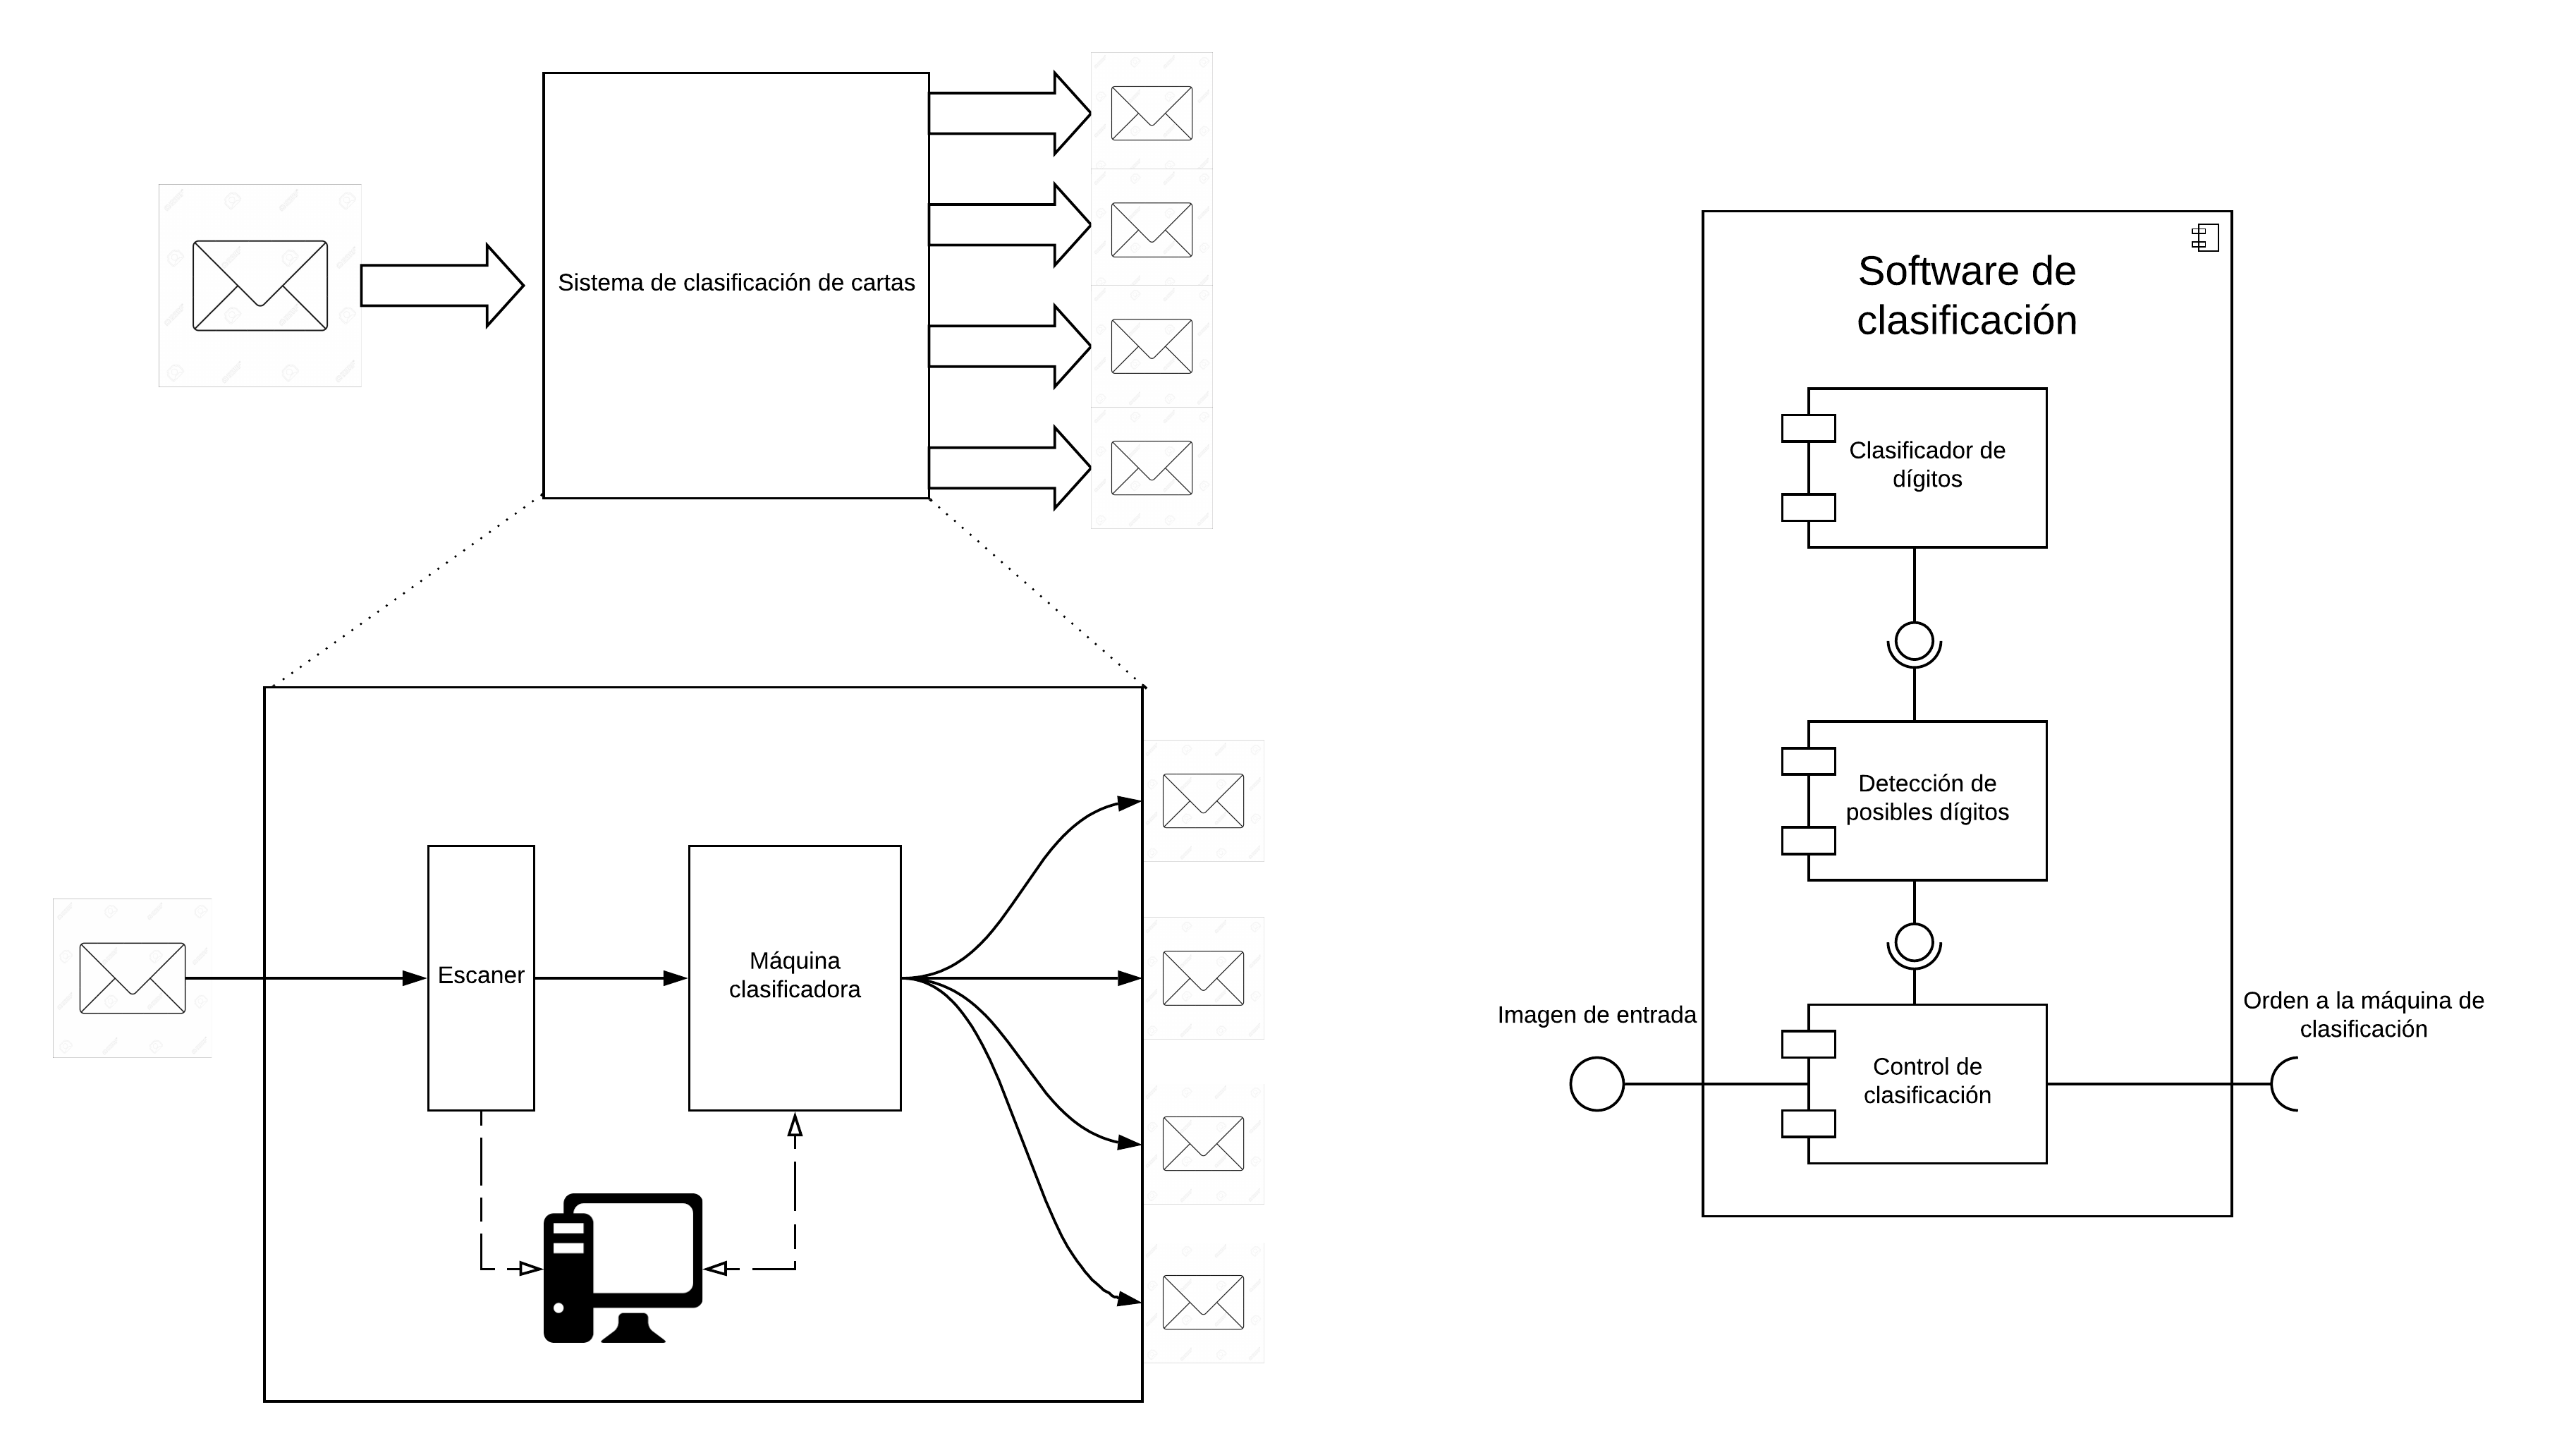
\includegraphics[scale=0.52]{figure/cartas.png}
	\caption{Leer códigos postales y clasificar cartas}
\end{figure}


Se propone un sistema de clasificación de cartas que recibe las cartas por una entrada, las clasifica y las devuelve por diferentes salidas dependiendo de su código postal.\\

\textbf{El sistema consiste en}\\
•	Un sistema de bandas transportadoras que lleva las cartas a través del sistema.\\
•	Un escáner, que digitaliza el código postal.\\
•	Una máquina clasificadora, que envía la carta por el camino adecuado mediante un sistema de bandas transportadoras.\\
•	Una computadora conectada al escáner y a la máquina clasificadora, que controla dicha máquina haciendo uso de un software de clasificación.\\

\textbf{El software de clasificación contiene los siguientes componentes:}\\
•	Un proceso de control de clasificación: recibe la imagen desde el escáner, y controla la máquina clasificadora. El control de clasificación llama a un proceso de detección de dígitos para que le traduzca el código postal.\\
•	El proceso de detección de dígitos: detecta los posibles dígitos separados de la imagen, y solicita a un proceso clasificador de dígitos que le clasifique dicho dígito. Con todos los dígitos obtenidos arma el código postal para enviarlo al control de clasificación.\\
•	El proceso clasificador de dígitos: hace uso del modelo de clasificación de redes nuronales (Modelo 2) para clasificar cada imagen como un dígito, y devolverle dicho dígito al proceso de detección de dígitos.\\

\section{Repositorio}

Repositorio en GitHub con el código R del trabajo y el Informe. \\
\href{https://github.com/hebermudezg/Clasificacion-de-digitos-MNIST}

\section{Conclusiones}

Las redes neuronales resultan ser una de las herramientas mas poderosas en el tema de clasificación de imágenes puesto que presentan un rendimiento muchas veces mejor que otras metodologías convencionales de clasificación tanto así que el análisis de imágenes con redes neuronales representa un campo en pleno auge llamado visión artificial, donde  se estudia estas metodologías para llevarlas a la industria de manera eficiente como por ejemplo en la conducción autos autónomos que reconocen el ambiente que los rodea mediante redes neuronales que procesan imágenes para ser muy seguros.  

\section{Bibliografía}

\begin{description}
\textbf{Introducción a los Modelos de Clasificación en R} \\
tomado de: https://rpubs.com/rdelgado/397838 \\
\\
\textbf{Redes neuronales convolucionales} \\
tomado de: https://es.wikipedia.org/wiki/Redes\_neuronales\_convolucionales \\
\\
\textbf{MNIST Handwritten Digit Recognition in Keras}\\
tomado de: https://nextjournal.com/gkoehler/digit\-recognition\-with\-keras \\
\\
\textbf{Handwritten Digit Prediction using Convolutional Neural Networks} \\
tomado de: https://medium.com/coinmonks/handwritten\-digit\-prediction\-using\-convolutional\-neural\-networks\-in\-tensorflow\-with\-keras\-and\-live\-5ebddf46dc8 \\
\\
\textbf{RStudio Team: (2019). Integrated Development for R. RStudio, Inc., Boston, MA URL} \\
http://www.rstudio.com/.

\end{description}

\end{document}
 
